% Options for packages loaded elsewhere
\PassOptionsToPackage{unicode,linktoc=all,pdfpagemode=FullScreen,bookmarks=true}{hyperref}
\PassOptionsToPackage{hyphens}{url}
\PassOptionsToPackage{dvipsnames,svgnames,x11names}{xcolor}
%
\documentclass[
  letterpaper,
  toc=chapterentrywithdots,
  11pt,
  headings=small]{scrreprt}

\usepackage{amsmath,amssymb}
\usepackage{iftex}
\ifPDFTeX
  \usepackage[T1]{fontenc}
  \usepackage[utf8]{inputenc}
  \usepackage{textcomp} % provide euro and other symbols
\else % if luatex or xetex
  \usepackage{unicode-math}
  \defaultfontfeatures{Scale=MatchLowercase}
  \defaultfontfeatures[\rmfamily]{Ligatures=TeX,Scale=1}
\fi
\usepackage{lmodern}
\ifPDFTeX\else  
    % xetex/luatex font selection
    \setmainfont[Path=./engine/misc/Times/,Extension=.ttf,UprightFont=*,BoldFont=*
Bold]{Times New Roman}
    \setsansfont[Path=./engine/misc/Times/,Extension=.ttf,UprightFont=*,BoldFont=*
Bold]{Times New Roman}
\fi
% Use upquote if available, for straight quotes in verbatim environments
\IfFileExists{upquote.sty}{\usepackage{upquote}}{}
\IfFileExists{microtype.sty}{% use microtype if available
  \usepackage[]{microtype}
  \UseMicrotypeSet[protrusion]{basicmath} % disable protrusion for tt fonts
}{}
\makeatletter
\@ifundefined{KOMAClassName}{% if non-KOMA class
  \IfFileExists{parskip.sty}{%
    \usepackage{parskip}
  }{% else
    \setlength{\parindent}{0pt}
    \setlength{\parskip}{6pt plus 2pt minus 1pt}}
}{% if KOMA class
  \KOMAoptions{parskip=half}}
\makeatother
\usepackage{xcolor}
\usepackage[margin=.75in,left=1in,right=1in,top=1in,bottom=3cm,footskip=2cm,marginparwidth=1in,marginparsep=0.75cm]{geometry}
\setlength{\emergencystretch}{3em} % prevent overfull lines
\setcounter{secnumdepth}{5}
% Make \paragraph and \subparagraph free-standing
\makeatletter
\ifx\paragraph\undefined\else
  \let\oldparagraph\paragraph
  \renewcommand{\paragraph}{
    \@ifstar
      \xxxParagraphStar
      \xxxParagraphNoStar
  }
  \newcommand{\xxxParagraphStar}[1]{\oldparagraph*{#1}\mbox{}}
  \newcommand{\xxxParagraphNoStar}[1]{\oldparagraph{#1}\mbox{}}
\fi
\ifx\subparagraph\undefined\else
  \let\oldsubparagraph\subparagraph
  \renewcommand{\subparagraph}{
    \@ifstar
      \xxxSubParagraphStar
      \xxxSubParagraphNoStar
  }
  \newcommand{\xxxSubParagraphStar}[1]{\oldsubparagraph*{#1}\mbox{}}
  \newcommand{\xxxSubParagraphNoStar}[1]{\oldsubparagraph{#1}\mbox{}}
\fi
\makeatother


\providecommand{\tightlist}{%
  \setlength{\itemsep}{0pt}\setlength{\parskip}{0pt}}\usepackage{longtable,booktabs,array}
\usepackage{calc} % for calculating minipage widths
% Correct order of tables after \paragraph or \subparagraph
\usepackage{etoolbox}
\makeatletter
\patchcmd\longtable{\par}{\if@noskipsec\mbox{}\fi\par}{}{}
\makeatother
% Allow footnotes in longtable head/foot
\IfFileExists{footnotehyper.sty}{\usepackage{footnotehyper}}{\usepackage{footnote}}
\makesavenoteenv{longtable}
\usepackage{graphicx}
\makeatletter
\def\maxwidth{\ifdim\Gin@nat@width>\linewidth\linewidth\else\Gin@nat@width\fi}
\def\maxheight{\ifdim\Gin@nat@height>\textheight\textheight\else\Gin@nat@height\fi}
\makeatother
% Scale images if necessary, so that they will not overflow the page
% margins by default, and it is still possible to overwrite the defaults
% using explicit options in \includegraphics[width, height, ...]{}
\setkeys{Gin}{width=\maxwidth,height=\maxheight,keepaspectratio}
% Set default figure placement to htbp
\makeatletter
\def\fps@figure{htbp}
\makeatother

\usepackage{tabularray}
\usepackage{booktabs}
\usepackage{tabularx}
\usepackage{mdframed}
\usepackage[acronym,toc,nomain]{glossaries}
\usepackage{todonotes}
\usepackage{threeparttable}

\RedeclareSectionCommand[
  beforeskip=0pt,
  afterindent=false% <- added
]{chapter}
\setkomafont{chapter}{\fontsize{14}{16.8}\selectfont}
\setkomafont{section}{\fontsize{12}{14}\selectfont}   
\setkomafont{subsection}{\fontsize{12}{14}\selectfont}
%\usepackage{tocloft}

\newglossarystyle{mystyle}
{
    \setglossarystyle{long3colheader}%
    \renewcommand*{\glossaryheader}{
    %  \textbf{Notation} & \textbf{Description} &
      \vspace{8pt}
    \endhead}%
    \renewcommand*{\glossaryname}{}
    \renewcommand*{\entryname}{}
    \renewcommand*{\pagelistname}{}
   % \renewcommand*{\descriptionname}{\textbf{Description}}
    \renewcommand{\glossentry}[2]{%
       \glsentryitem{##1}\glstarget{##1}{\glossentryname{##1}}
        & \glossentrydesc{##1}
        & ##2
        \tabularnewline*}%
}
\makeatletter
\@ifpackageloaded{bookmark}{}{\usepackage{bookmark}}
\makeatother
\makeatletter
\@ifpackageloaded{caption}{}{\usepackage{caption}}
\AtBeginDocument{%
\ifdefined\contentsname
  \renewcommand*\contentsname{Table of contents}
\else
  \newcommand\contentsname{Table of contents}
\fi
\ifdefined\listfigurename
  \renewcommand*\listfigurename{Figures in-text}
\else
  \newcommand\listfigurename{Figures in-text}
\fi
\ifdefined\listtablename
  \renewcommand*\listtablename{Tables in-text}
\else
  \newcommand\listtablename{Tables in-text}
\fi
\ifdefined\figurename
  \renewcommand*\figurename{Figure}
\else
  \newcommand\figurename{Figure}
\fi
\ifdefined\tablename
  \renewcommand*\tablename{Table}
\else
  \newcommand\tablename{Table}
\fi
}
\@ifpackageloaded{float}{}{\usepackage{float}}
\floatstyle{ruled}
\@ifundefined{c@chapter}{\newfloat{codelisting}{h}{lop}}{\newfloat{codelisting}{h}{lop}[chapter]}
\floatname{codelisting}{Listing}
\newcommand*\listoflistings{\listof{codelisting}{List of Listings}}
\makeatother
\makeatletter
\makeatother
\makeatletter
\@ifpackageloaded{caption}{}{\usepackage{caption}}
\@ifpackageloaded{subcaption}{}{\usepackage{subcaption}}
\makeatother

\ifLuaTeX
  \usepackage{selnolig}  % disable illegal ligatures
\fi
\usepackage{bookmark}

\IfFileExists{xurl.sty}{\usepackage{xurl}}{} % add URL line breaks if available
\urlstyle{same} % disable monospaced font for URLs
\hypersetup{
  pdftitle={Population Pharmacokinetic Report},
  pdfauthor={MMJ},
  colorlinks=true,
  linkcolor={blue},
  filecolor={Maroon},
  citecolor={Blue},
  urlcolor={Blue},
  pdfcreator={LaTeX via pandoc}}


\usepackage[headsepline,footsepline]{scrlayer-scrpage}
\usepackage{cleveref}
\pagestyle{scrheadings}
\lohead{Population PK Report \\ Report No.: }
\rohead{DRAFT}
\ifoot{CONFIDENTIAL}
\ofoot{22 Sep 2024} % empty 
\cfoot{Page \thepage}

\renewcommand*\chapterpagestyle{scrheadings}

\renewcommand{\glsnamefont}[1]{#1}

\setlength\LTleft{0pt}
\setlength\LTright{0pt}
\setlength\glsdescwidth{0.8\hsize}
\loadglsentries{}
\setglossarystyle{mystyle}
\makenoidxglossaries
\begin{document}
% TODO: Add custom LaTeX header directives here
\thispagestyle{empty}
\vskip2cm
{\centerline{\textbf{POPULATION PHARMACOKINETICS REPORT}}}
\vskip1cm
\begin{table}[!h]
      \setlength{\tabcolsep}{5pt}
      \renewcommand{\arraystretch}{1.5}
      \begin{tabularx}{\textwidth}{|p{0.3\textwidth}|X|}
            \hline
            \textbf{Report Number:} & \\
            \hline
            \textbf{Report Title:} & Population Pharmacokinetic
Report \\
            \hline
            \textbf{Study Drug:} &  Drug A\\
            \hline
            \textbf{Indication(s):} & Nothing\\
            \hline
            \textbf{Study Number(s):} & 12345\\
            \hline
            \textbf{Sponsor:} & \\
            \hline
            \textbf{Prepared By:} & MMJ\\
            \hline
            \textbf{Reviewed By:} & MMJ \\
            \hline
            \textbf{Approved By:} & MMJ\\
            \hline
            \textbf{Report Date:} & 22 Sep 2024\\
            \hline
            \textbf{Report Status:}  & DRAFT\\
            \hline
      \end{tabularx}
\end{table}
\vskip0.5cm
\begin{center}
{\textbf{CONFIDENTIAL}}
\begin{mdframed}
    {\normalsize This is a Company Name. document that contains
confidential information. It is intended solely for the recipient and
must not be disclosed to any other party. This material may be used only
for evaluating or conducting clinical investigations; any other proposed
use requires written consent from Company Name.}
\end{mdframed}
\end{center}

\renewcommand*\contentsname{Contents}
{
\hypersetup{linkcolor=blue}
\setcounter{tocdepth}{2}
\tableofcontents
}
\listoffigures
\listoftables

\bookmarksetup{startatroot}

\chapter{}\label{section}

\bookmarksetup{startatroot}

\chapter{EXECUTIVE SUMMARY}\label{sec-executive-summary}

\textit{{Drug X, an oral tablet which is being developed by company A and is used to treat Disease Y, has undergone N number of completed studies. A population PK analysis was performed to characterize the PK and identify sources of variability in the PK  based on rich and sparse samples collected in Phase 1 and Phase 3 studies. As part of the population PK analysis, data from NN subjects was utilized where the doses were ranging from 5 mg- 100 mg Q3W.
The data was adequately described using a 1-compartment model with a first-order absorption rate constant (Ka) with lag time (Tlag). A bootstrap method resulted in model reduction compared to reducing the full model with the additional of all the covariates like (age, sex, baseline body weight, race, baseline GFR, drug product)  by removing covariates for which the 95% PIs included the null value relative to the reference compared stepwise covariate modeling using forward addition and backward elimination. Both continuous and categorical variables were evaluated and. The final population estimates of CL/F and V/F for drug X were 19.49 L/h and 198.72 L, respectively, and are for a male patient who is 92.5 kg, has a CRCL of 116.5 mL/min, and is taking a dose of 150 mg. Based on the population PK model, the half-life of drug X was 7.07 The effect of creatinine clearance was added on CL/F since the drug was previously demonstrated as important  as Drug X is expected to undergo renal excretion. Baseline body weight of each subjects was modeled as covariate on the CL, VC using a power function and the the estimates are  respectively.Sex was a significant covariate on CL and VC (Figure 6), with male subjects having a higher CL and higher Vc than female subjects.
Final Model-based simulations were performed to evaluate drug X CL under various conditions, estimate effective half-life, predict exposure metrics for 60 mg Q4W vs 30 mg Q2W dose regimens, and assess the clinical relevance of covariates of interest such as sex, hepatic function, renal function, race, manufacture process, and shorter infusion time in the final PPK model. Results suggest that exposures were higher in female subjects than males for subjects who received 60 mg Q4W. The predicted geometric means of drug X exposure (Cmin1, Cmax1, Cavg1, Cavd28, Cminss, Cmaxss, and Cavgss) at 60 mg Q4W and 30 mg Q2W are summarized in Table 5.  As expected, Cavgss was similar across the two different regimens (difference < 5%). The exposures were higher with drug X 30 mg Q2W relative to 60 mg Q4W by approximately 51% for Cmind28 and 42% for Cminss. The exposures were lower with drug X 30 mg Q2W relative to 60 mg Q4W by approximately 50% for Cmax1 and 31% for Cmaxss, which were also expected.
}}

\bookmarksetup{startatroot}

\chapter*{SYNOBSIS}\label{sec-synobsis}
\addcontentsline{toc}{chapter}{SYNOBSIS}

\markboth{SYNOBSIS}{SYNOBSIS}

\bookmarksetup{startatroot}

\chapter{INTRODUCTION}\label{sec-introduction}

\section{Exploratory Data Analysis}\label{exploratory-data-analysis}

\section{PK Plots}\label{pk-plots}

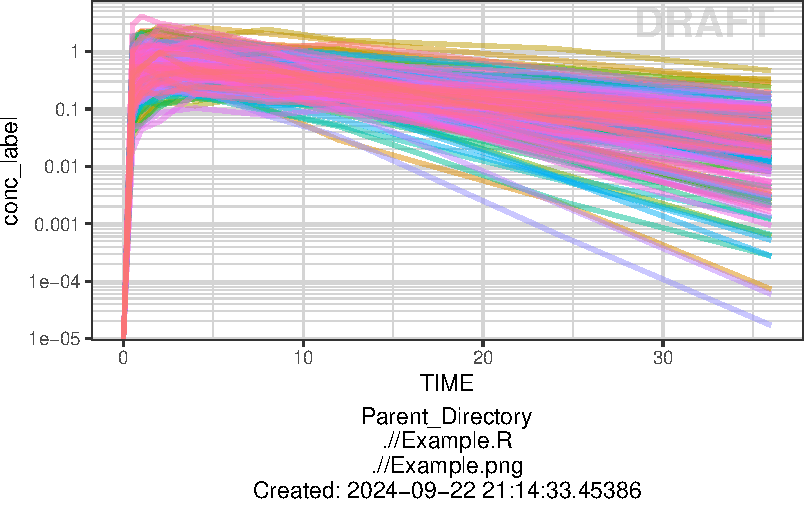
\includegraphics{sec/introduction_files/figure-pdf/unnamed-chunk-2-1.pdf}

\section{Covariate Summary}\label{covariate-summary}

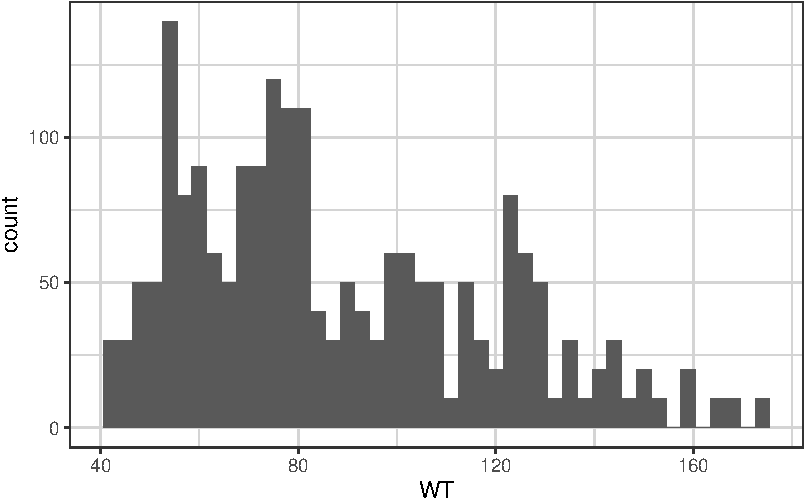
\includegraphics{sec/introduction_files/figure-pdf/unnamed-chunk-3-1.pdf}

\bookmarksetup{startatroot}

\chapter{METHODS}\label{sec-methods}

\bookmarksetup{startatroot}

\chapter{RESULTS}\label{sec-results}

For each analysis (e.g.~PopPK, PK/PD analysis, exposure-response
analysis and simulations), an own sub-section should be included.

\section{Exploratory Data Analysis}\label{exploratory-data-analysis-1}

Concentration-time profiles of drug X following oral administration of
the first dose on Day 1 in healthy subjects are presented in Figure 2.
Additional concentration-time profiles of drug X are presented in
Appendix 2. A list of samples excluded from the analysis is presented in
Appendix 2. Drug X was rapidly absorbed following oral administration
and declined in a multi-exponential manner. Doses ranged from 5 mg to
100 mg. Drug X exposure was dose proportional, and the accumulation
ratio based on 80 mg once daily dosing was 1.3 in Study 123.

\section{Model Development}\label{model-development}

\subsection{Base Model}\label{base-model}

A population PK analysis was performed based on rich and sparse samples
collected in Phase 1 and Phase 3 studies in order to identify the
structural model. Highlights of the base population PK analysis are
presented below and in Appendix 2. 1- and 2-compartment models with
linear elimination were tested. The 1-compartment model resulted in the
lowest OFV. A first-order absorption rate constant (Ka) with lag time
(Tlag) was used to characterize the rapid absorption of drug X. A mixed
error model (additive and proportional) resulted in a substantially
lower OFV relative to proportional or additive error models. Additional
model refinements are presented below. An allometric function accounting
for body weight effect on clearance (CL/F) and volume of distribution
(V/F) was included in the model (run008). In addition, the effect of
creatinine clearance was added on CL/F since the drug was previously
demonstrated to undergo important renal excretion (run019).

\begin{verbatim}

Looking for NONMEM table files.
    Reading ./sdtab1 
    Reading ./patab1 
    Reading ./cotab1 
Table files read.
    Reading ./run1.phi 

Looking for NONMEM simulation table files.
No simulated table files read.
\end{verbatim}

\begin{verbatim}

Reporting transformed parameters:
For the OMEGA and SIGMA matrices, values are reported as standard deviations for the diagonal elements and as correlations for the off-diagonal elements. The relative standard errors (RSE) for OMEGA and SIGMA are reported on the approximate standard deviation scale (SE/variance estimate)/2. Use `transform = FALSE` to report untransformed parameters.

Estimates for $prob no.1, subprob no.1, method foce
 Parameter  Label    Value      RSE
 THETA1     CL       9.996      0.03791
 THETA2     V        109.1      0.04173
 THETA3     KA       0.9377     0.04867
 THETA4     PROP ERR 0.2021     0.02284
 OMEGA(1,1) PPV_CL   0.5285     0.04845
 OMEGA(2,1)          0.5713     0.07815
 OMEGA(2,2) PPV_V    0.5701     0.04943
 OMEGA(3,3) PPV_KA   0.642      0.07221
 SIGMA(1,1)          1      fix  - 
\end{verbatim}

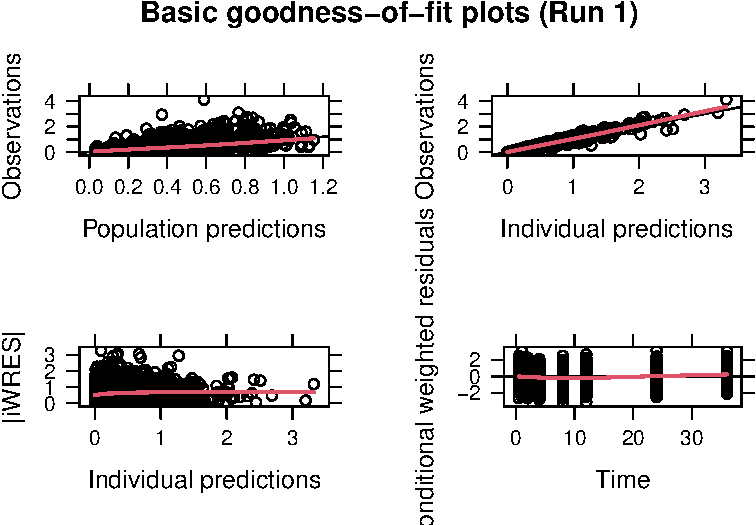
\includegraphics{sec/results_files/figure-pdf/unnamed-chunk-2-1.pdf}

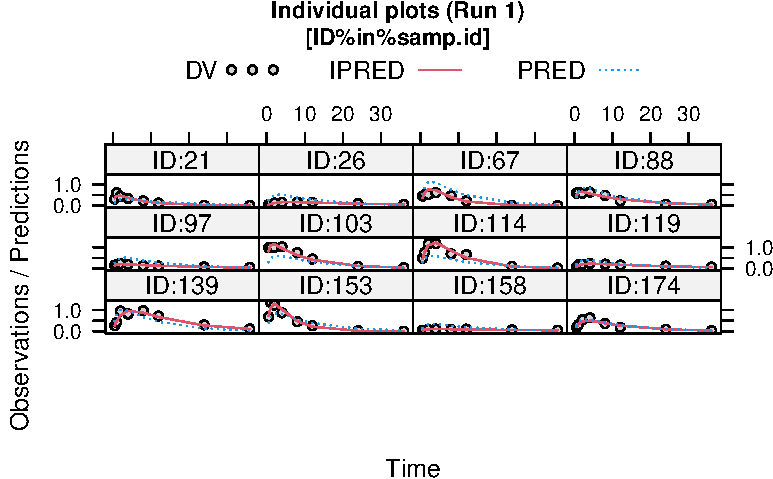
\includegraphics{sec/results_files/figure-pdf/unnamed-chunk-2-2.pdf}

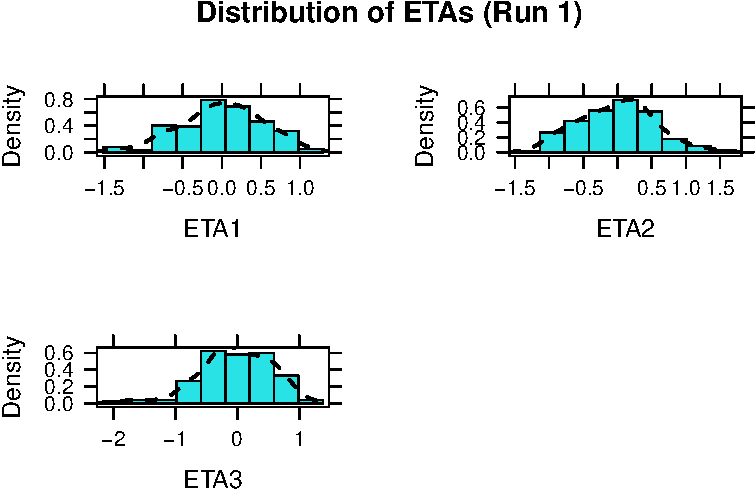
\includegraphics{sec/results_files/figure-pdf/unnamed-chunk-2-3.pdf}

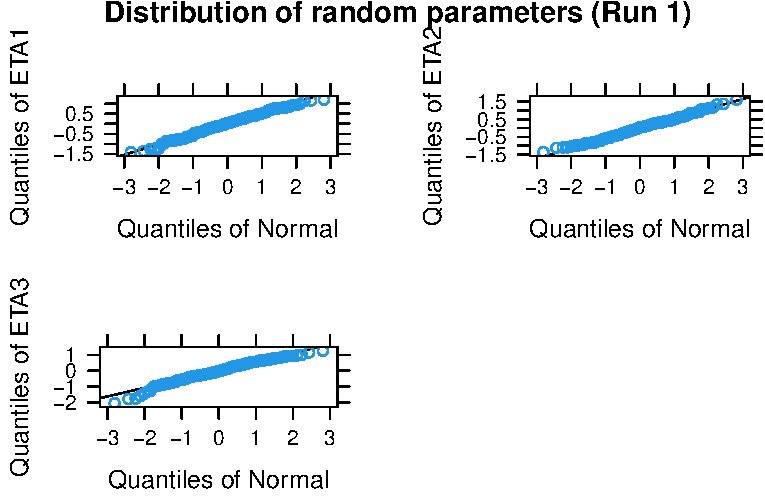
\includegraphics{sec/results_files/figure-pdf/unnamed-chunk-2-4.pdf}

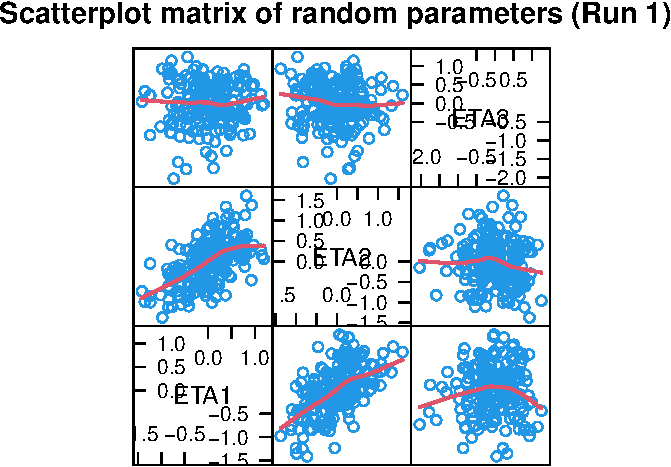
\includegraphics{sec/results_files/figure-pdf/unnamed-chunk-2-5.pdf}

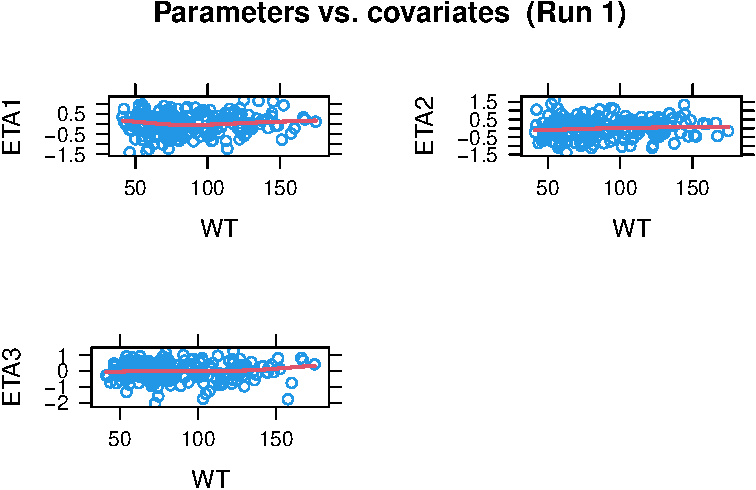
\includegraphics{sec/results_files/figure-pdf/unnamed-chunk-2-6.pdf}

\subsection{Covariate Model}\label{covariate-model}

Potential relationships between PK parameters (random effects) of drug X
and categorical and continuous covariates from the base PK model
(run019) are presented in Appendix 2. A stepwise covariate analysis was
performed to identify sources of variability in PK parameters of drug X.
Results for covariate analysis are presented in Appendix 2. A summary of
covariates resulting in the maximum reduction of the OFV and included in
each step of the analysis is presented in Table 6.

Covariates were evaluated using a forward inclusion approach with
p\textless0.01 (ΔOFV\textgreater6.6349). The effect of fasted status on
Ka resulted in the most important decrease in OFV as part of the first
step of the analysis (ΔOVF = -322.051). In the second step, the effect
of dose on CL/F resulted in the most important decrease in OFV (ΔOVF =
-161.224). In the 3rd and 4th steps, the effect of gender on V/F and
CL/F resulted in the most important decrease in OFV (ΔOVF = -50.805and
-72.726, respectively). In the 5th step, the effect of ESRD on CL/F
resulted in the most important decrease in OFV (ΔOVF = -16.624). In the
6th step, the effect of dose on Ka resulted in the most important
decrease in OFV (ΔOVF = -71.311). In the 7th step, the effect of
formulation Ka resulted in the most important decrease in OFV (ΔOVF =
-21.636). In the 8th step, the effect of disease status (healthy
subjects vs.~narcolepsy/OSA patients) resulted in the most important
decrease in OFV (ΔOVF = -17.684). Additional information is available in
Appendix 2 (Section 12.36). During the backward testing, none of the
covariate were removed. Additional information is available in Appendix
2. The bootstrap method was used to reduce the full model by removing
covariates for which the 95\% PIs included the null value relative to
the reference population. Based on the estimates of the population PK
model, concentration-time profiles of drug X were simulated (1000
replicates). Statistically significant covariates were retained in the
reduced final model if the nonparametric 95\% PIs excluded the null
value relative to the reference population. All the covariates tested in
the full model resulted in a statistically significant effect, and were
retained in the final model.

\begin{longtable}[]{@{}rlrrr@{}}
\caption{Covariate Model Results}\tabularnewline
\toprule\noalign{}
Step & Covariates & Base\_OFV & New\_OFV & ΔOFV \\
\midrule\noalign{}
\endfirsthead
\toprule\noalign{}
Step & Covariates & Base\_OFV & New\_OFV & ΔOFV \\
\midrule\noalign{}
\endhead
\bottomrule\noalign{}
\endlastfoot
1 & Fasted status on Ka & 93576 & 93254 & -322 \\
2 & Dose on CL/F & 93254 & 93092 & -161 \\
3 & Gender on V/F & 93092 & 93042 & -50 \\
4 & Dose on Ka & 93042 & 92969 & -72 \\
5 & Formulation on Ka & 92881 & 92859 & -21 \\
6 & Disease Status on CL/F & 92859 & 92842 & -17 \\
\end{longtable}

\subsection{Final Model}\label{final-model}

Typical population PK parameters of drug X derived with the final model
(run005) are presented in Table 7. The continuous covariates (CRCL and
weight) were centered to a reference value in the population PK analysis
(116.5 mL/min and 92.5 kg). The reference value is \textless1\%
different than the median value in the Phase 3 studies.

The population estimates of CL/F and V/F for drug X were 19.49 L/h and
198.72 L, respectively, and are for a male patient who is 92.5 kg, has a
CRCL of 116.5 mL/min, and is taking a dose of 150 mg. Based on the
population PK model, the half-life of drug X was 7.07 h.

\begin{verbatim}

Looking for NONMEM table files.
    Reading ./sdtab2 
    Reading ./patab2 
    Reading ./cotab2 
Table files read.
    Reading ./run2.phi 

Looking for NONMEM simulation table files.
No simulated table files read.
\end{verbatim}

\begin{verbatim}

Reporting transformed parameters:
For the OMEGA and SIGMA matrices, values are reported as standard deviations for the diagonal elements and as correlations for the off-diagonal elements. The relative standard errors (RSE) for OMEGA and SIGMA are reported on the approximate standard deviation scale (SE/variance estimate)/2. Use `transform = FALSE` to report untransformed parameters.

Estimates for $prob no.1, subprob no.1, method foce
 Parameter  Label    Value      RSE
 THETA1     CL       11.35      0.04252
 THETA2     V        129.2      0.04959
 THETA3     KA       0.9373     0.0487
 THETA4     PROP ERR 0.2021     0.02282
 OMEGA(1,1) PPV_CL   0.5954     0.05392
 OMEGA(2,1)          0.6779     0.05134
 OMEGA(2,2) PPV_V    0.6847     0.04548
 OMEGA(3,3) PPV_KA   0.6431     0.07359
 SIGMA(1,1)          1      fix  - 
\end{verbatim}

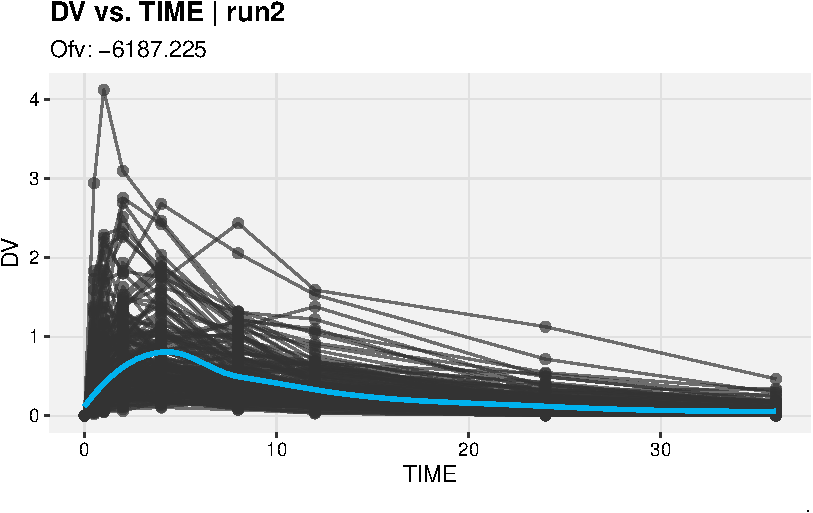
\includegraphics{sec/results_files/figure-pdf/unnamed-chunk-4-1.pdf}

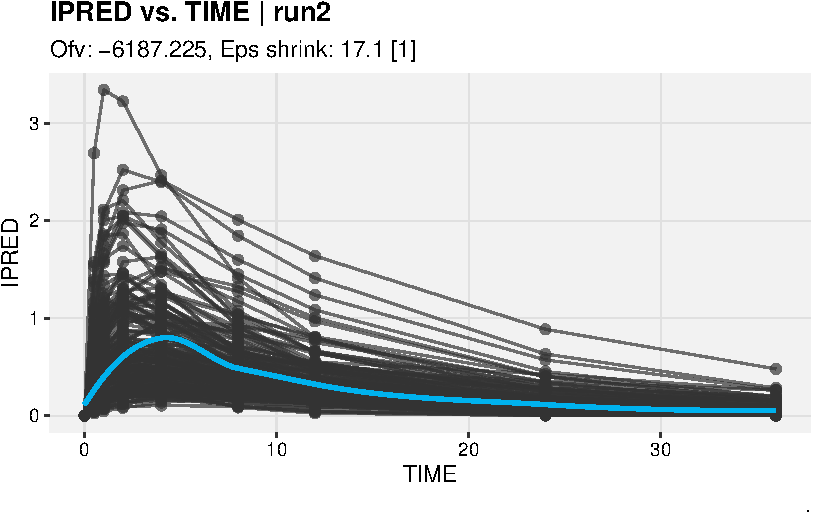
\includegraphics{sec/results_files/figure-pdf/unnamed-chunk-4-2.pdf}

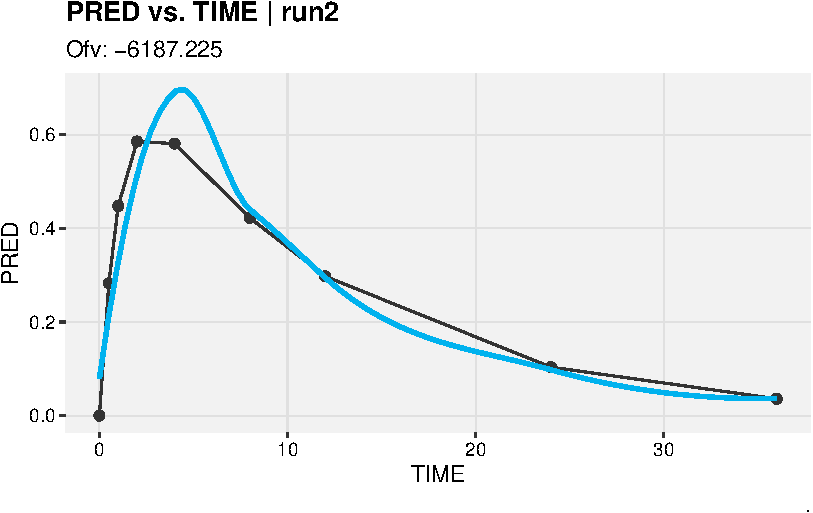
\includegraphics{sec/results_files/figure-pdf/unnamed-chunk-4-3.pdf}

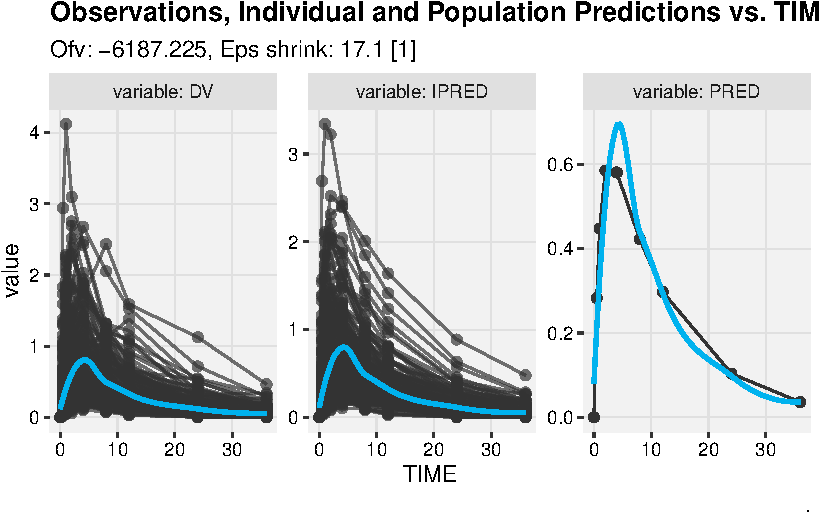
\includegraphics{sec/results_files/figure-pdf/unnamed-chunk-4-4.pdf}

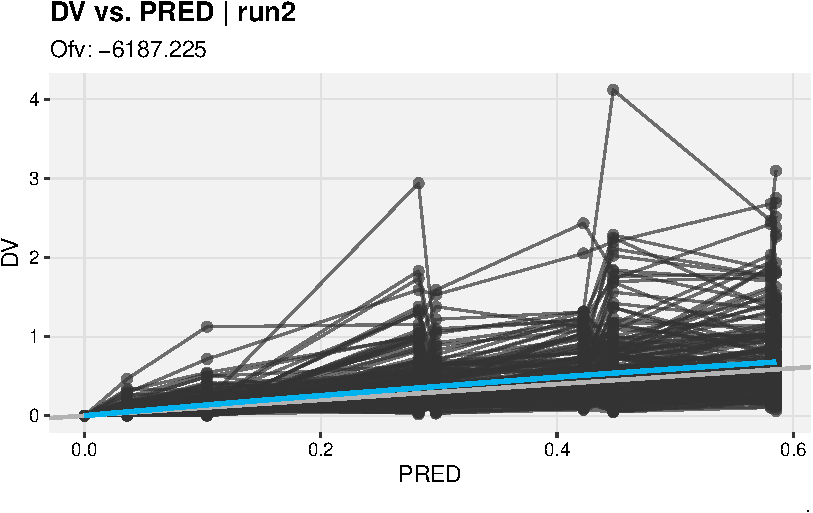
\includegraphics{sec/results_files/figure-pdf/unnamed-chunk-4-5.pdf}

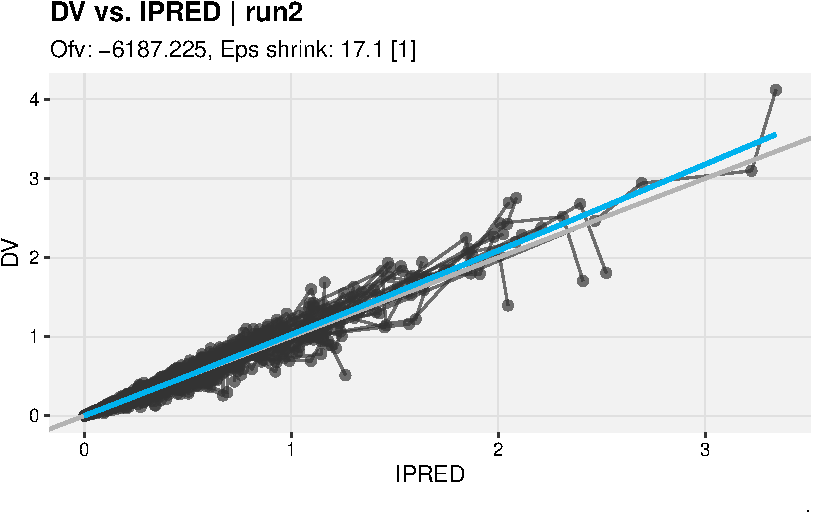
\includegraphics{sec/results_files/figure-pdf/unnamed-chunk-4-6.pdf}

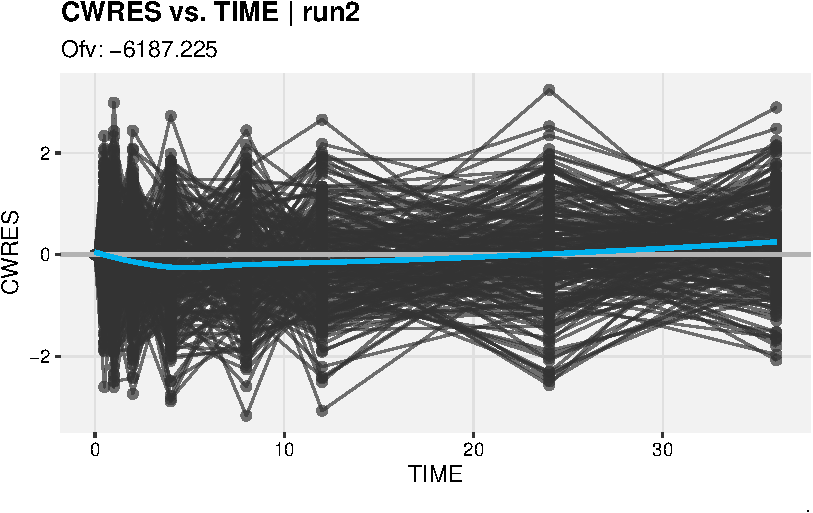
\includegraphics{sec/results_files/figure-pdf/unnamed-chunk-4-7.pdf}

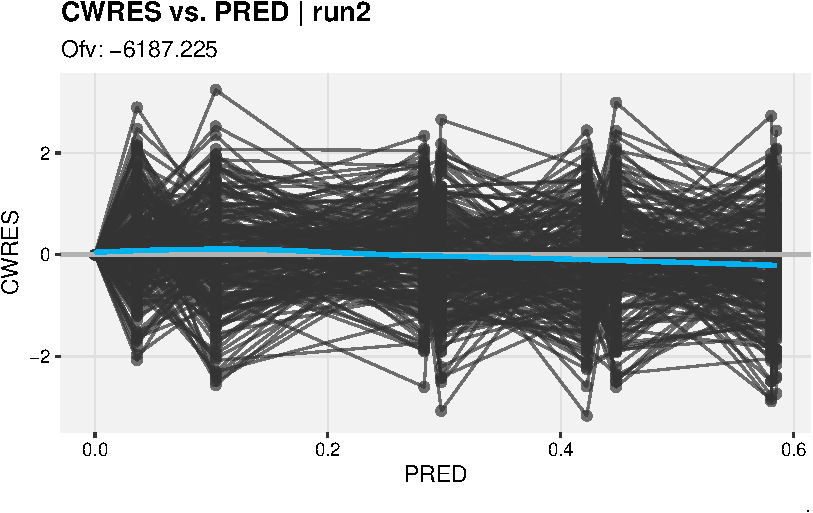
\includegraphics{sec/results_files/figure-pdf/unnamed-chunk-4-8.pdf}

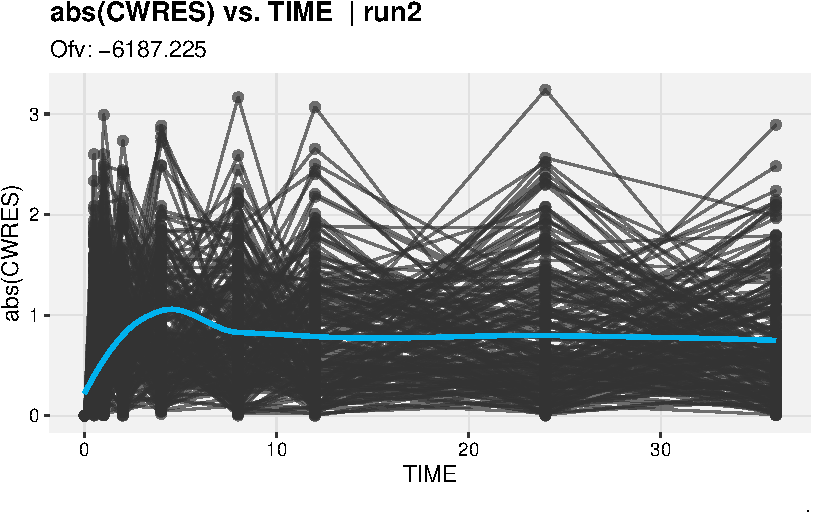
\includegraphics{sec/results_files/figure-pdf/unnamed-chunk-4-9.pdf}

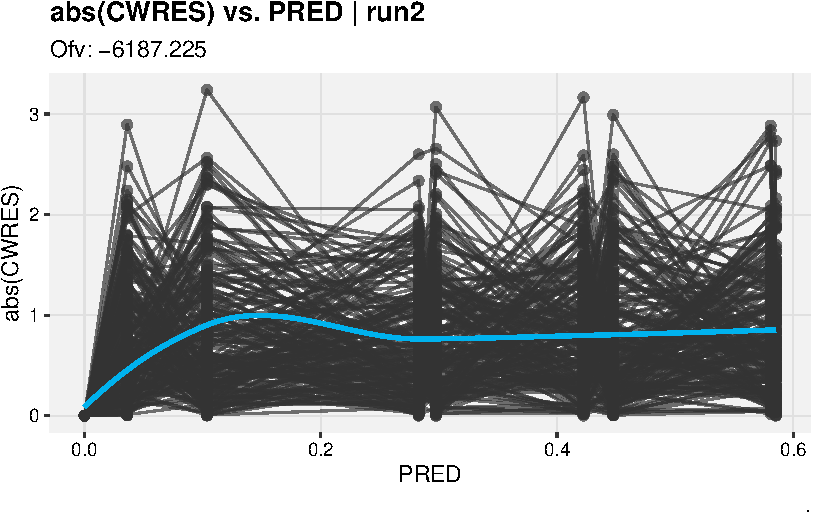
\includegraphics{sec/results_files/figure-pdf/unnamed-chunk-4-10.pdf}

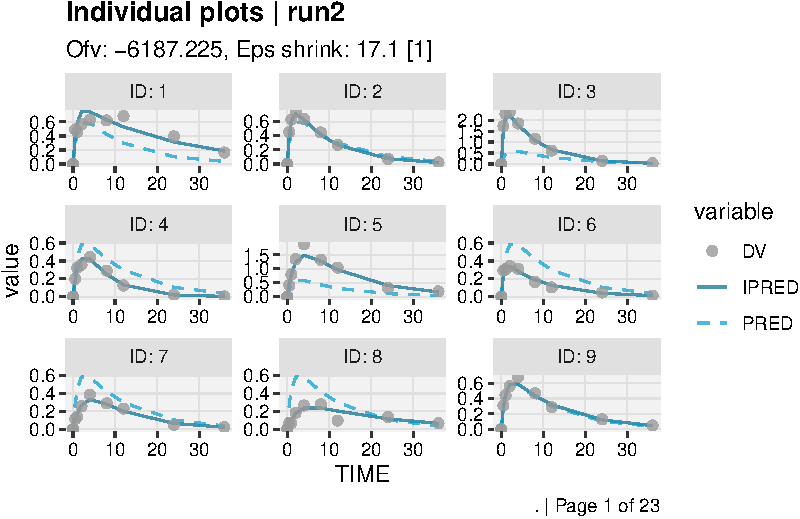
\includegraphics{sec/results_files/figure-pdf/unnamed-chunk-4-11.pdf}

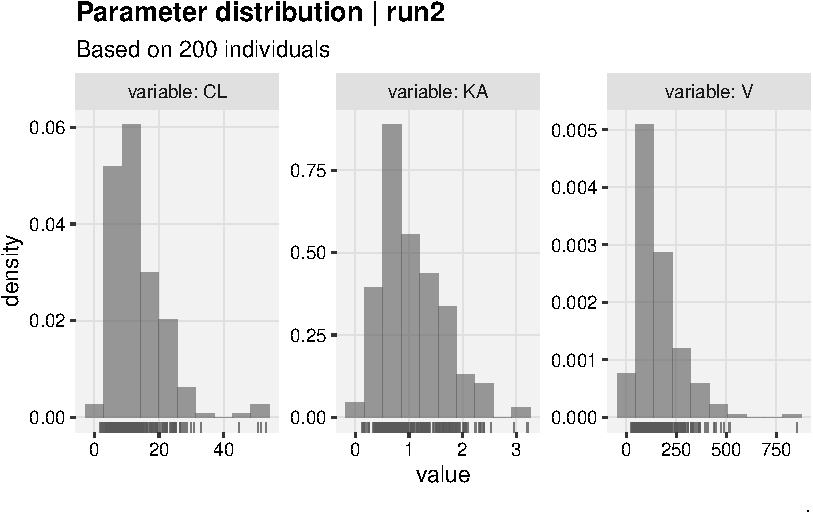
\includegraphics{sec/results_files/figure-pdf/unnamed-chunk-4-12.pdf}

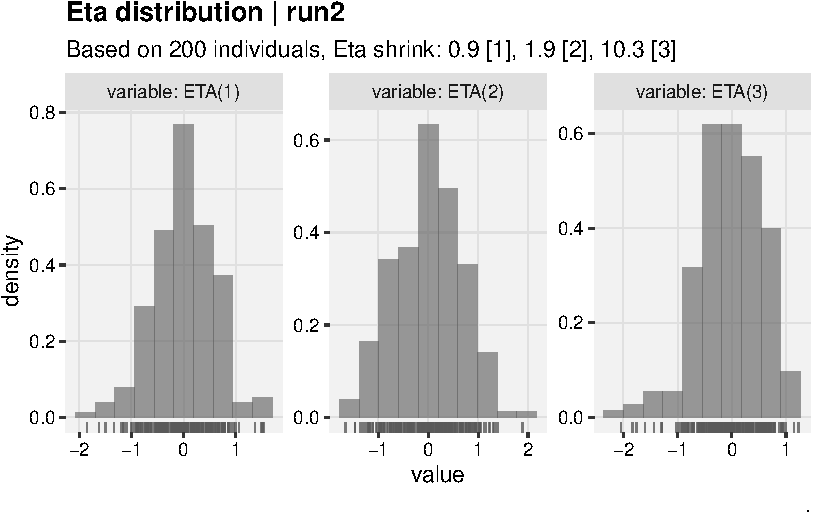
\includegraphics{sec/results_files/figure-pdf/unnamed-chunk-4-13.pdf}

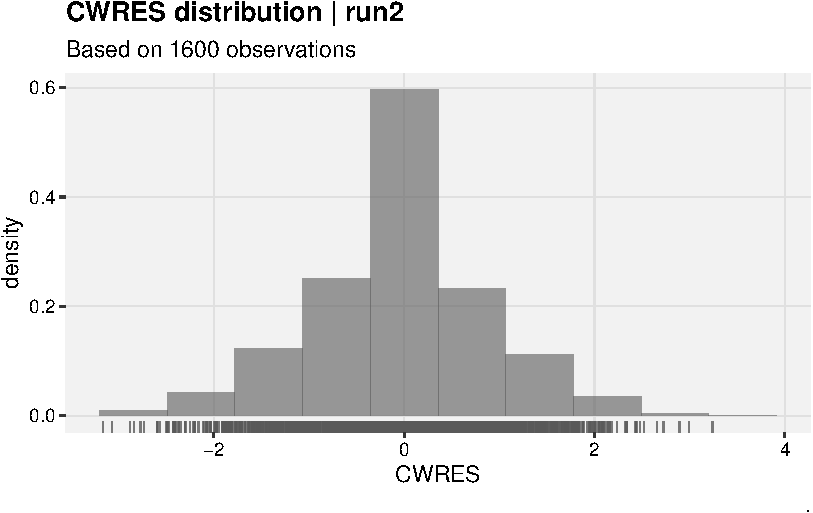
\includegraphics{sec/results_files/figure-pdf/unnamed-chunk-4-14.pdf}

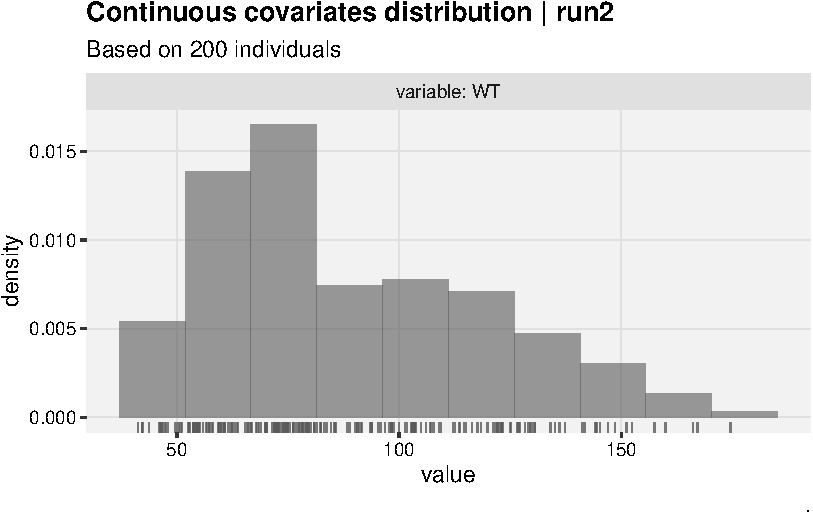
\includegraphics{sec/results_files/figure-pdf/unnamed-chunk-4-15.pdf}

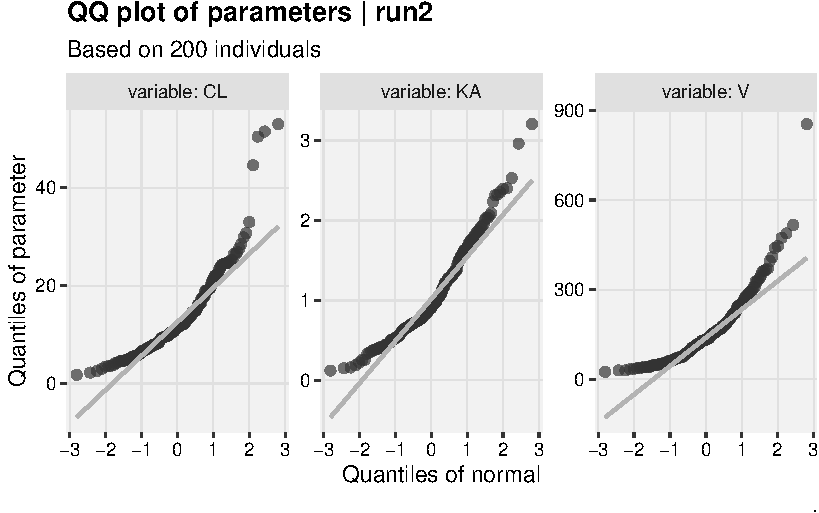
\includegraphics{sec/results_files/figure-pdf/unnamed-chunk-4-16.pdf}

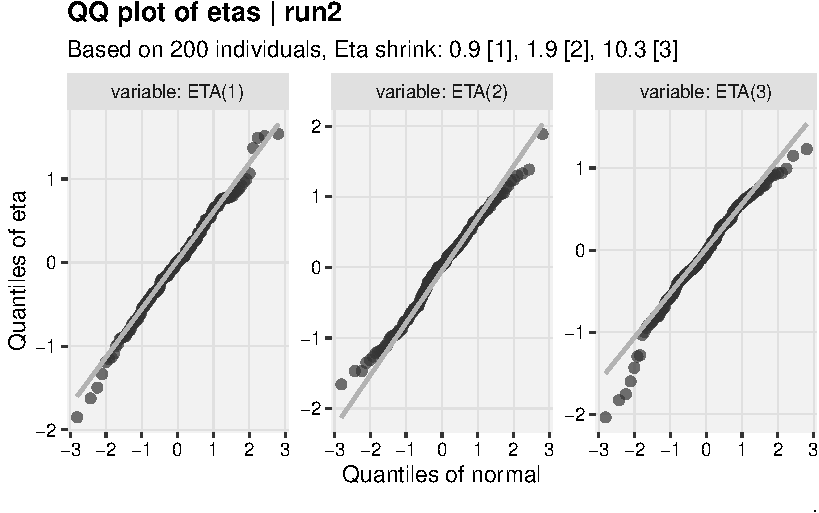
\includegraphics{sec/results_files/figure-pdf/unnamed-chunk-4-17.pdf}

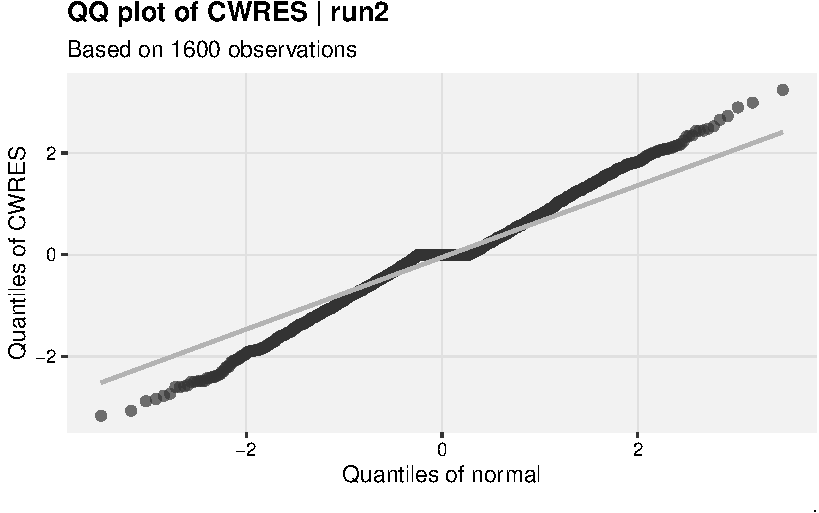
\includegraphics{sec/results_files/figure-pdf/unnamed-chunk-4-18.pdf}

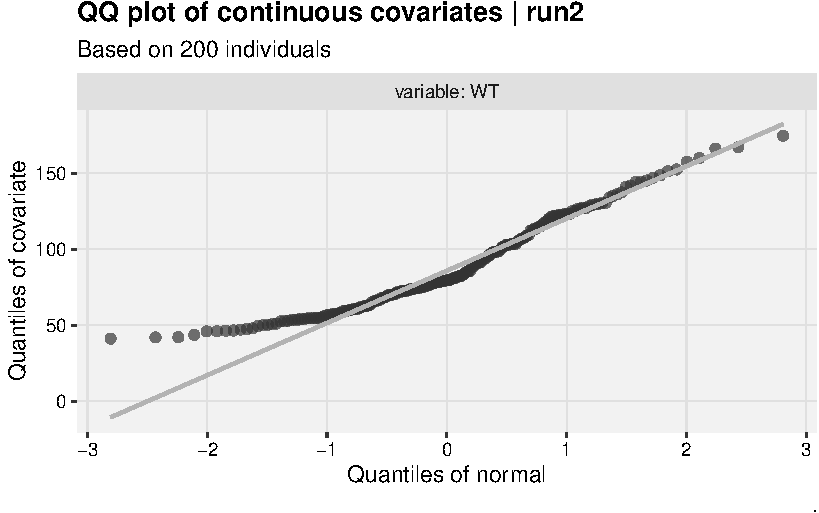
\includegraphics{sec/results_files/figure-pdf/unnamed-chunk-4-19.pdf}

\section{Model Evaluation}\label{model-evaluation}

Visual predictive checks were performed for the full PPK model
stratified by patient population and dosing regimens, and the results
are in Figure 5. Overall, the pcVPC results indicate that the model
adequately characterized the data and predicted concentrations to be
used for E-R efficacy and safety analyses. The observed 5th, 50th
(median), and 95th percentiles generally fall within the 90\% PI (the
shaded band) up to the first 60 days after the previous dose and the
first 600 days after the first dose (trough concentrations). A pcVPC
stratified by body weight is provided in Appendix 3.

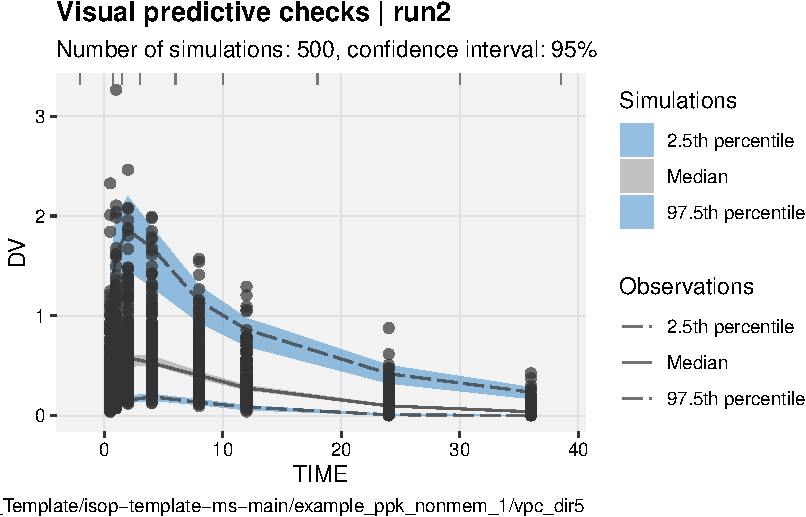
\includegraphics{sec/results_files/figure-pdf/unnamed-chunk-5-1.pdf}

\section{Model Application}\label{model-application}

Model-based simulations were performed to evaluate drug X CL under
various conditions, estimate effective half-life, predict exposure
metrics for 60 mg Q4W vs 30 mg Q2W dose regimens, and assess the
clinical relevance of covariates of interest such as sex, hepatic
function, renal function, race, manufacture process, and shorter
infusion time in the final PPK model. The final model was used in these
simulations.

\subsection{Covariate Model Evaluation of Effect of
Sex}\label{covariate-model-evaluation-of-effect-of-sex}

Sex was a significant covariate on CL and VC (Figure 6), with male
subjects having a higher CL and higher Vc than female subjects.
Comparisons of model predicted drug exposure at 60 mg Q4W by sex are
presented in Figure 6. In general, exposures were higher in female
subjects than males for subjects who received 60 mg Q4W.

Sex was a significant covariate on CL and VC (Figure 6), with male
subjects having a higher CL and higher Vc than female subjects.
Comparisons of model predicted drug exposure at 60 mg Q4W by sex are
presented in Figure 6. In general, exposures were higher in female
subjects than males for subjects who received 60 mg Q4W.

\subsection{Covariate Model Comparison of 30 mg Q2W and 60 Q4W
Regimens}\label{covariate-model-comparison-of-30-mg-q2w-and-60-q4w-regimens}

The predicted geometric means of drug X exposure (Cmin1, Cmax1, Cavg1,
Cavd28, Cminss, Cmaxss, and Cavgss) at 60 mg Q4W and 30 mg Q2W are
summarized in Table 5. As expected, Cavgss was similar across the two
different regimens (difference \textless{} 5\%). The exposures were
higher with drug X 30 mg Q2W relative to 60 mg Q4W by approximately 51\%
for Cmind28 and 42\% for Cminss. The exposures were lower with drug X 30
mg Q2W relative to 60 mg Q4W by approximately 50\% for Cmax1 and 31\%
for Cmaxss, which were also expected.

\bookmarksetup{startatroot}

\chapter{DISCUSSION}\label{sec-discussion}

\bookmarksetup{startatroot}

\chapter{CONCLUSION}\label{sec-conclusion}

Summary of major findings. Contextualize the PK model based simulations
with regard to therapeutic window ?

\bookmarksetup{startatroot}

\chapter{REFERENCES}\label{references}

\bookmarksetup{startatroot}

\chapter{}\label{section-1}

\cleardoublepage
\phantomsection
\addcontentsline{toc}{part}{Appendices}
\appendix

\chapter{SI-01}\label{si-01}




\end{document}
